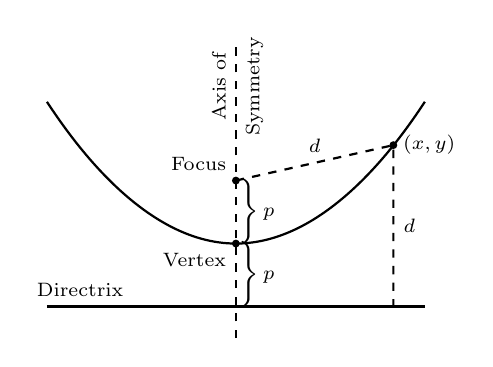
\begin{tikzpicture}[scale=.8]
	
	\draw [thick,{\colorone}] (-3,-1) node [above,black,shift={(12pt,0pt)}] {\scriptsize Directrix} %node [below,black,shift={(12pt,0pt)}] {\scriptsize $y=-p$} 
	-- (3,-1);
	
	\filldraw [black] (0,1) circle (1.5pt) node [above left] {\scriptsize Focus};% node [below ] {\scriptsize $F=(0,p)$};
	\draw [thick,{\colortwo}](-3,2.25) parabola bend (0,0) (3,2.25);
	\filldraw (0,0) circle (1.5pt) node [below left] {\scriptsize Vertex};
	\draw (.3,.5) node[] {\scriptsize $\left.\rule{0pt}{12pt}\right\}p$};
	\draw (.3,-.5) node[] {\scriptsize $\left.\rule{0pt}{12pt}\right\}p$};
	
	\coordinate (A) at (2.5,1.5625);
	\filldraw [black] (A) circle (1.5pt) node [right] {\scriptsize $(x,y)$};
	\draw [thick,dashed](0,1) -- (A) node [pos=.5,above] {\scriptsize $d$} -- (2.5,-1) node [pos=.5,right] {\scriptsize $d$};
	
	\draw [thick,dashed] (0,-1.5) -- node [pos=.85,above,rotate=90] {\scriptsize Axis of} node [pos=.85,below,rotate=90] {\scriptsize Symmetry} (0,3.2);
	
\end{tikzpicture}
